\documentclass[12pt]{article}

\usepackage{xspace}
\newcommand{\eg}{e.g.\@\xspace}
\newcommand{\ie}{i.e.\@\xspace}
\newcommand{\normal}{\mathcal{N}}
\newcommand{\GEV}{\operatorname{GEV}}
\newcommand{\iid}{i.i.d.\@\xspace}
\makeatletter
\newcommand*{\etc}{%
    \@ifnextchar{.}%
        {etc}%
        {etc.\@\xspace}%
}
\makeatother

\newcommand{\expectation}{\ensuremath{\mathbb{E}}}
\newcommand{\variance}{\ensuremath{\mathbb{V}}}
\newcommand{\probability}{\ensuremath{\mathbb{P}}}
\newcommand{\invlogit}{\ensuremath{\text{logit}^{-1}}}
% Packages With Options
\usepackage[letterpaper, margin=1in]{geometry} % page
\usepackage[english]{babel} % language
\usepackage[utf8]{inputenc} % input
\usepackage[inline]{enumitem} 
\usepackage[section]{placeins} % floats appear in the section they were defined in

% Other Package calls
\usepackage{
  array, % for fixed-width tables
  amssymb, amsmath, % for math
  authblk, % for authors
	booktabs, % for nice tables
  csquotes, % better biblatex
  graphicx, % for figures
  indentfirst, % indent the first line
  physics, % for physics notation
  ragged2e, % for better alignment of text
  siunitx, % for SI notation
  nth, % for 1st, 2nd, 3rd, nth
}

% PACKAGE SETTINGS
\setlength{\RaggedRightParindent}{\parindent} % fix ragged right
\graphicspath{{fig/}{../../fig/}}
\sisetup{round-mode=figures,round-precision=3,scientific-notation=false}
\allowdisplaybreaks{} % let the align environment span multiple pages

% arrays with fixed width
\newcolumntype{L}[1]{>{\raggedright\let\newline \\ \arraybackslash\hspace{0pt}}m{#1}}

\title{Climate Change Adaptation: Uncertainty Associated with Sequential Finite Period Decisions under Nonstationarity}
\author[1,2]{James Doss-Gollin}
\author[1,2]{Upmanu Lall}
\author[1,2]{David Farnham}
\affil[1]{Columbia Water Center, Columbia University}
\affil[2]{Department of Earth and Environmental Engineering, Columbia University}

\usepackage[hidelinks]{hyperref}
\usepackage{cleveref}
\usepackage[
  backend=biber,
  doi=true,
  url=false,
  isbn=false,
  style=authoryear-comp,
  %style=nature,
  natbib=true,
  backref=false,
  maxbibnames=3,
  maxcitenames=2,
  uniquename=false,
  uniquelist=false,
  sorting=ynt
]{biblatex}
\renewcommand{\refname}{References}
\renewbibmacro{in:}{}
\AtEveryBibitem{\clearfield{month}\clearfield{pages}}

\addbibresource{../library.bib}

% -----------------------------------------------------------------------------
% AUTHOR AND TITLE AND TITLEPAGE
% -----------------------------------------------------------------------------

\begin{document}
\maketitle
\RaggedRight{}
\begin{abstract}
  Hydroclimatic systems exhibit organized low-frequency and regime-like variability at multiple time scales, causing the risk associated with climate extremes such as floods and droughts to vary at multiple timescales.
  Despite broad recognition of this nonstationarity, there has been little theoretical development of ideas for the design and operation of infrastructure that simultaneously consider the potential for predictability of secular change and regime behavior or low-frequency variability.
  Consequently, existing theories of flood risk assessment are well-suited to analysis of flood adaptation strategies with fixed project operation period \(M\), but not for analysis of sequential decision strategies.
  In this paper we illustrate some basic considerations of uncertainty and risk analysis associated with the sequential decisions that may need to be made for climate risk adaptation in a nonstationary adaptation.
  We simulate synthetic data and fit the resulting simulations in a Bayesian context using stationary and non-stationary models to show that \(\ldots{}\).
  This is a first conceptual step to the development of a full sequential decision analysis approach under nonstationarity.
\end{abstract}


\section{Introduction}

Hydroclimatic systems vary on many timescales, including regime-like variability and secular variability  \citep{Milly2008,Merz2014,Hurst1951,Sveinsson2005,Hodgkins2017,Matalas2012}.
This multi-scale variability greatly complicates the estimation of future flood sequences, leading to ``low confidence in projections of changes in fluvial floods'' \citep{IPCC2012}.
Yet the same memory and low-frequency variability that complicate projecting flood sequences far into the future may also impart some predictability at short timescales \citep{Jain2001}.
The existence of this information gap suggests that approaches for adapting to hydroclimate risks, such as floods, which have short project operation periods, may be preferential in some cases to large and permanent projects with long project operations.

Classical methods for design of infrastructure first specify a return period \(T\) (\ie{} 100 years), and then design a project that protects against this \(T\)-year event.
The mathematical problem of interest then becomes estimation of the probability distribution \( f(p_T) \), where \( p_T \) is binary event that the threshold \( Q_T \) is exceeded by the annual-maxiumum flood series \( Q(t) \):
\begin{equation*}
  p_T(t) \equiv \probability \qty[ Q(t) \geq Q_T] \qqtext{for} t = \qty[t_0 + 1, \ldots, t_0 + M]
\end{equation*}
where \( t_0 \) is the first year forecast and \( M \) is the project operation period.
Although in a stationary setting an unbiased estimator of \( P \qty[ Q(t) \geq Q_T] \) converges asymtotically to \(1 - \frac{1}{T}\), the asymmetric uncertainty distribution of the estimate has also prompted the consideration of the potential for over- or under-design for floods if the conditional mean of the estimated distribution of \( Q_T \) is used for design \citep{Stedinger1997}\footnote{Manu has mentioned a Vogel198x citation but I haven't successfully found it.}.

\subsection{Physical Reasoning}

In order to make probabilistic predictions of future flooding in a particular location, it is helpful to begin by considering the specific physical mechanisms which may lead to flooding in particular location.

In large river basins, extreme river flooding typically requires the large-scale transport and convergence of moisture\citep{Lu2013,Merz2014,Dacre2014}\footnote{Farnham et al}, which often requires specific climate mechanisms.
For example, major river floods in the Ohio River Basin (USA) in the 20th century exhibit remarkably consistent large-scale circulation features in the weeks preceding the flood peak \citep{Nakamura2012,Robertson2015}.
This is consistent with findings that have linked flood risk around the world with well-known climate mechanisms such as El Ni\~{n}o-Southern Oscillation (ENSO) \citep{Ward2014,Emerton2017}.

Nonstationarity in hydroclimate systems can occur due to climate change, river modification, and land use change \citep{Milly2008,Merz2014}.
Thermodynamic scaling arguments predict an intensified hydrologic cycle under global warming due to the Clausius-Clapeyron scaling of the atmosphere's moisture-holding capacity with temperature \citep[see][]{Muller2011,OGorman2015}.
However, these scaling arguments do not in general hold over land \citep{Byrne2015,Shaw2016}.
In addition to thermodynamical changes, climate extremes are highly sensitive to changes in future climate dynamics, which are themselves imperfectly understood due to complex and non-linear physics \citep{Palmer2013}.
Consequently, predicting future flood risk in a particular location involves making estimates of future climate circulation patterns, the associated thermodynamics, as well as any catchment- and river-scale changes which may affect rainfall-runoff response.

\subsection{Estimating Future Flood Risk}

Under classical assumptions of stationarity, all estimates are assumed independent of time.
Yet even under stationarity, \citet{Jain2001} showed that low-frequency variability can lead to a high probability of surprise, particularly when the length of the record used for estimation \(N\) is short.
This finding is particularly important to keep in mind given that low-frequency change has been found to be large as compared to detected trends in the observed record \citep{Hodgkins2017}.

Attempts to use a ``model chain'' approach emcompassing:
\begin{enumerate*}[label= (\roman*) ]
  \item emission scenario;
  \item general circulation model (GCM);
  \item downscaling;
  \item hydrological catchment model; and
  \item flood frequency analysis,
\end{enumerate*}
typically with bias correction applied at several steps, can lead to results which are difficult to interpret in a probabilistic context \citep{Dankers2009,Ott2013,Merz2014,Dittes2017}.

In particular, the downscaling and bias correction methods typically applied assume stationary relationships (\eg{} between GCM rainfall and observed rainfall) which have no physical basis, particularly in a changing climate.
Recent work has also sought to shorten the above model chain by modeling \( Q(X(t)) \), where\( X \) is a set of climate state variables from a GCM run, and where the relationship between \(X\) and \(Q\) can more reasonably be assumed stationary \citep{Hall2014,Delgado2014,Silva2016}.
Alternatively, purely statistical approaches have extended classical flood frequency analysis by incorporating a time trend in the parameters of statistical distributions \citep{Obeysekera2014,Vogel2011,Serinaldi2015,Strupczewski2001}.
In this case, however, the analyst can choose not only the distribution but also  the time parameterization, if any, for each parameter, leading to many researcher degrees of freedom \citep[``forking paths'' or ``multiple comparisons'';][]{Gelman2013} and exacerbating the problems caused by lack of theory for model choice even under nonstationarity \citep{Kidson2016}.

To capture this influence, some recent studies have incorporated a climate index or set of climate indices \(X\) as predictor variables for streamflow \citep{Delgado2014,Silva2016,Sun2014,Griffis2007}\footnote{Farnham et al}.
For a more comprehensive review, we refer the reader to \citet{Hall2014}.\footnote{Farnham et al}


\subsection{Decision Approaches}

Incorporating uncertain projections of physical variables into useful decision models is further hampered by the diffulties inherent to forecasting the needs of society\footnote{Cite needed}, which may even be coupled to the natural system.\footnote{Insert citation on socio-hydrology}
Risk-based design methods \citep[RBDM; see][]{Rosner2014} recognize that the appropriate level of design  may itself be a decision variable.
\citet{Lall1987} considered the uncertainty in the frequency with which floods may exceed the design level for different values of \(p\) (equivalent to different values of \(T\)), and also for different sample sizes for estimation \(N\) and different project operation periods \(M\).
Some prominent methodologies for risk-based design under nonstationary in the water resources literature include robust decision making (RDM)\footnote{(Lempert et al. 2006; Lempert and Groves 2010; Matrosov et al. 2013)}, scenario-neutral planning\footnote{(Prudhomme et al. 2010)}, infogap analysis\footnote{(Ben-Haim 2006; Korteling et al. 2013)}, and decision scaling\footnote{(Brown et al. 2011, 2012; Moody and Brown 2013; Turner et al. 2014)}. 

Alternatively, sequential decision models \citep[see][]{Russell2003,Howard1960} allow decision-makers to optimize not only what action to take, but also when to take it.
Sequential decision models have been used in the hydrological literature for sea wall optimization \citep{Lickley2014}
\texttt{need some citations for sequential decisions}.
Given that, low-frequency variability or system memory may lead to less uncertain probabilistic forecasts at short times than long times, models which can capture this uncertainty may be particularly advantageous for sequential models.

There is thus \emph{a critical theoretical need for decision frameworks which can compare projects of different operation period} using an arbitrary choice of model of future flood behavior.
In the following sections we illustrate some basic considerations of uncertainty and risk analysis associated with the sequential decisions that may need to be made for climate risk adaptation in a nonstationary environment.
Understanding the full uncertainty associated with thresholds of interest is relevant to many other climate adaptation problems, including infrastructure design for flood management, because we are faced with the task of estimating the infrastructure's probability of failure \(p_T\) for the next \(M\) years, as well as the uncertainty and bias in this estimate.
This is a first conceptual step to the development of a full sequential decision analysis approach under nonstationarity.

We proceed as follows \(\ldots{}\)

\section{Methods}\label{sec:methods}

We use an idealized model to generate sequences of annual-maximum floods, fit these sequences in a probabilistic framework to three flood models that incorporate time in different ways, and evalaluate the performance of these models for multiple observational record lengths \(N\) and project planning periods \(M\).

\subsection{Synthetic Flood Sequence Generation}

ENSO \citep[see][for a comprehensive review]{Sarachik2010} varies in a quasi-oscillatory manner with variability on the order of \SIrange{4}{6}{year} modulated by low-frequency behavior.
Though the time scales are specific to ENSO, this pattern of quasi-oscillatory behavior modulated by low-frequency behavior is typical of many other climate phenomena.
A \SI{100000}{year} integration of the Cane-Zebiak model \citep{Zebiak1987} was used to produce a monthly NINO3.4 index\footnote{We greatfully acknowledge the contribution of Nandini Ramesh} with stationary forcing.
To create an annual time series, we average the May-July months to create a time series \( X(t) \) where \(t\) is taken in annual steps \(1, \ldots, \num{100000}\).

Though statistical models relating climate indices and streamflow maxima typically require strong assumptions (\ie{} a stationary relationship between predictor and predictand; see \texttt{Farnham et al}), this framework is the starting point of our synthetic flood generation approach.

\begin{equation} \label{eq:lognormal}
  \log Q(t) \big| \mu(t),\sigma(t) \sim \normal \qty(\mu(t), \sigma(t)).
\end{equation}
The parameters of the distribution vary in time according to the sampled NINO3 index denoted \( X(t) \) as well as time itself, representing secular trends:
\begin{equation}
  \mu(t) = \mu_0 + \beta X(t) + \gamma \qty(t - t_0)
\end{equation}
and a constant coefficient of variation
\begin{equation}
  \sigma(t) = \begin{cases} \alpha \mu(t) & \qqtext{if} \alpha \mu(t) \geq 0.01 \\ 0.01 & \qqtext{else} \end{cases}
\end{equation}

We partition \( \mu(t) \) into a dynamical component, driven by the variability of the climate predictor \(X(t)\), and a trend component, represented by a linear increase in time.
This trend component may represent changes in land use, global temperature change, or river modification \citep[see][]{Merz2014}.
Though this is a highly simplified model neglecting many important mechanisms, it enables us to generate many synthetic sequences of \(\qty[M + N]\) years which exhibit chaotic but organized quasi-periodic behavior (regime behavior or low-frequency variability) plus a trend term, thereby capturing many essential features of hydrological variability.
Because the computational cost is small, it is easy to generate sets of sequences.

In \cref{sec:sequence-realistic} we show sequences of streamflow generated by this model for some choices of parameters and discuss the processes which they can reasonably represent.

\subsection{Distributional Model\label{sec:estimation}}

Because we do not, in general, know the true distribution of annual-maximum floods, we compare a stationary and non-stationary parameterizations of the generalized extreme value (GEV) statistical distribution (eq.~\ref{eq:GEV}) for estimating the distribution of \(Q(t)\) for the future \(M\)-year period.
\begin{equation}
  \label{eq:GEV}
  f(x \big| \mu, \sigma, \xi) = \frac{1}{\sigma}
    \begin{cases}
      \qty[1 + \xi \frac{x - \mu}{\sigma}] ^ {(-\flatfrac{1}{\xi})-1} \exp \qty[-\qty(1+\xi \frac{x - \mu}{\sigma})^{\flatfrac{-1}{\xi}}], & \xi \neq 0 \\
      \exp \qty[-\frac{x-\mu}{\sigma}] \exp \qty[- \exp \qty(- \frac{x-\mu}{\sigma})], & \xi = 0
    \end{cases}
\end{equation}
Where \(\mu{}\) is the location parameter, \(\sigma{}\) is the shape parameter, and \(\xi{}\) is the scale parameter of the GEV distribution.
For each simulation, the first \(N\) years \(\qty(t=[t_0-N+1, \ldots, t_0])\) are treated as observations.
Then, once the appropriate time parameterization is selected (\cref{tab:model-fitting}), the parameters are fit in a Bayesian framework to fully represent the posterior uncertainty.
Computation is carried out in the \texttt{python} environment, with simulation using the \texttt{numpy} package \citep{vanderWalt2011} and fitting using the No-U-Turn Sampler (NUTS) \citep{Hoffman2014} as implemented in the \texttt{stan} probabilistic programming language \citep{Carpenter2016}.
Weak (uninformative) priors are chosen based on recommendations from \citet{Martins2000}; the exact parameterizations are described in following sections which describe specific experiments.

\subsection{Hidden Markov Model\label{sec:HMM}}

A Hidden Markov Model (HMM) is a statistical Markov model in which the system being modeled is assumed to be a Markov process with unobserved (\ie{} hidden) states \citep{Rabiner1986}.
The (unobserved) states evolve following a first-order Markov process, and the observed variable (\ie{} streamflow) depends only on the observed state.
As such, HMMs are a structured prediction method which extend general mixture models to sequences of data, where position in the sequence is relevant.
Because this structure allows the hidden state to represent hydroclimatological ``regimes'' \citep{Reinhold1982,Michelangeli1995,Merz2014}, HMMs have have been used extensively to model hydrological variables such as streamflow \citep{Bracken2016}.
HMMs have also been used to model the evolution of climate states such as ENSO.\footnote{Julian's work}

To supplement the distributional models described in \cref{sec:estimation}, we also fit observed streamflow sequences using a HMM as implemented in the python \texttt{pomegranate} package \citep{Schreiber2016}.
The model is fit to the \(N\) observed years of data using the Baum-Welch algorithm, assuming that the data follow a log-normal distribution conditional only on the state.
To choose the number of hidden states, a log probability score is used.
Future floods are estimated by simulating future states from the resulting matrix and then drawing floods log-normally using the estimated parameters.

\begin{table}[b]
  \begin{center}
    \begin{tabular}{L{1.0in} L{3.0in} L{1.5in}}
      \toprule
        Model Name & Description & Relevant Section \\
      \midrule
        stationary & \(Q \sim \GEV \qty(\mu, \sigma, \xi)\) & \cref{sec:estimation} \\
        location trend & \(Q \sim \GEV \qty(\mu_0 + \beta_\mu \qty(t-t_0), \sigma, \xi)\) & \cref{sec:estimation} \\
        HMM & log-normal Hidden Markov Model & \cref{sec:HMM} \\
      \bottomrule
    \end{tabular}
  \end{center}
  \caption{Summary of models used for fitting\label{tab:model-fitting}}
\end{table}


\subsection{Flood Estimation and Uncertainty}

Finally, we consider a contract in which an insurer agrees to pay the entire coverage cost \(C\) every time that the trigger threshold \(Q_T\) is exceeded.
Although \(Q_T\) is in general a decision variable, we treat it as fixed.
Then, using the posterior distribution of the parameters of the chosen statistical model (from \cref{tab:model-fitting}) we estimate the probability that \(Q(t) \geq Q_T\) for \(t \in \vb{t}\), which is equivalent to \(p_T(t)\).

For a particular year, the fair price for the insurance premium is \(\expectation \qty(p_T) C\).
However, there is typically also a risk premium associated with the policy that prices the uncertainty in this estimate (since the trigger \(Q_T\) is specified in the contract and thus not uncertain).
This risk premium is proportional to the variance of \(p_T\), or more generally to its uncertainty distribution.
The insurance premium for a particular year is thus
\begin{equation} \label{eq:premium}
  Z(t) = C \qty[\expectation \qty(p_T(t)) + R \variance \qty(p_T(t))]
\end{equation}
where \(R \geq 0\) is a coefficient describing the cost of tue uncertainty in the estimate of \(p_T(t)\).

In this paper we consider the price of a contract of \(M\) years to be simply the summed price of the contract for each individual year.
We assume that the discount rate is equal to inflation (\ie{} the inflation-adjusted discount rate is zero) for simplicity.
A more comprehensive pricing mechanism for the financial instrument could incorporate more or different information about the uncertainty in the estimate, and should consider the price of the \(M\) years as a portfolio (\ie{} should consider correlation between the different years).
Such an approach, however, is not necessary for this conceptual study.

\section{Are Generated Sequences Realistic?\label{sec:sequence-realistic}}

In this section we discuss the sequences of streamflow that are generated and look at their ACF, PACF, distribution, wavelet spectrum, \etc{} and compare to some that have been identified in the literature.

\begin{figure}
  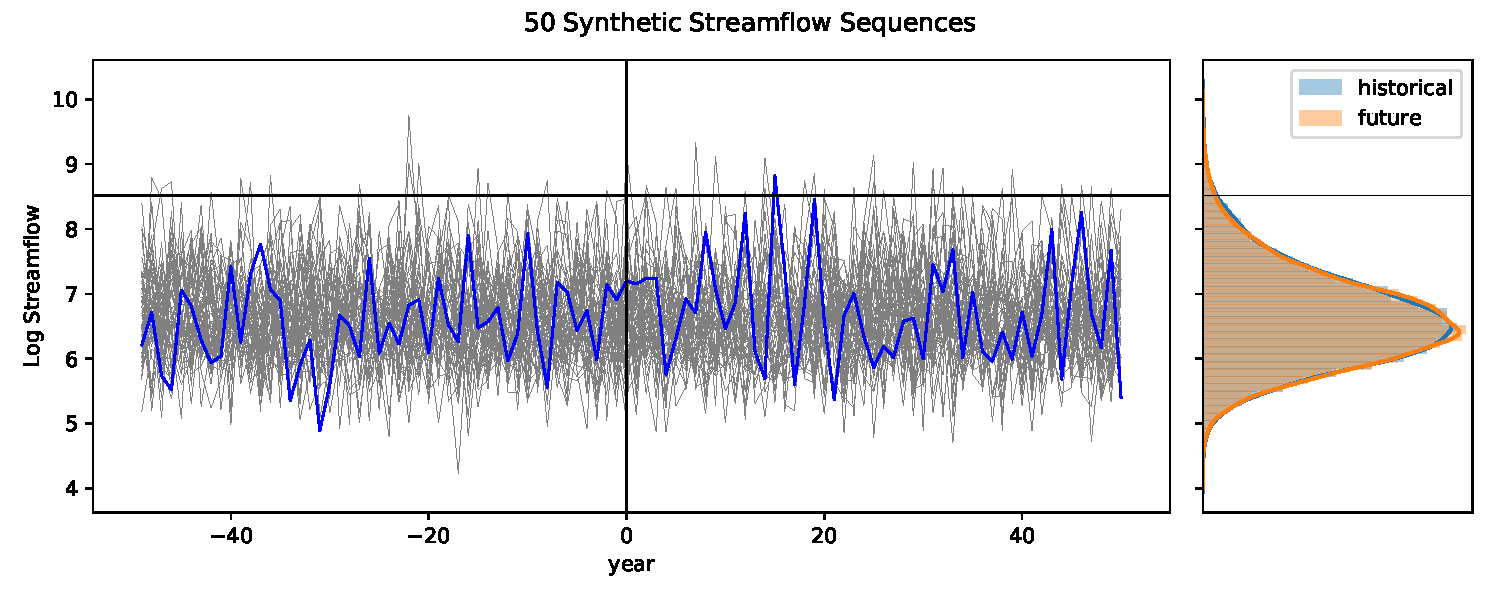
\includegraphics[width=\textwidth]{../../figs/stationary_sequences.pdf}
  \caption{50 simulated sequences created from the Cane-Zebiak model  \(N=50, M=50, t_0=0, \mu_0=6.5, \beta_\mu=0.5, \gamma=0, \alpha=0.075, \sigma_\text{min}=0.01\). 49 of the sequences are shown in gray and a single randomly chosen sequence is highlighted in blue for emphasis. (L) shows the time series of log streamflow as a function of year, while (R) shows the distribution of 500 sequences over the historical and future periods.}\label{fig:stationary-sequences}
\end{figure}

\begin{figure}
  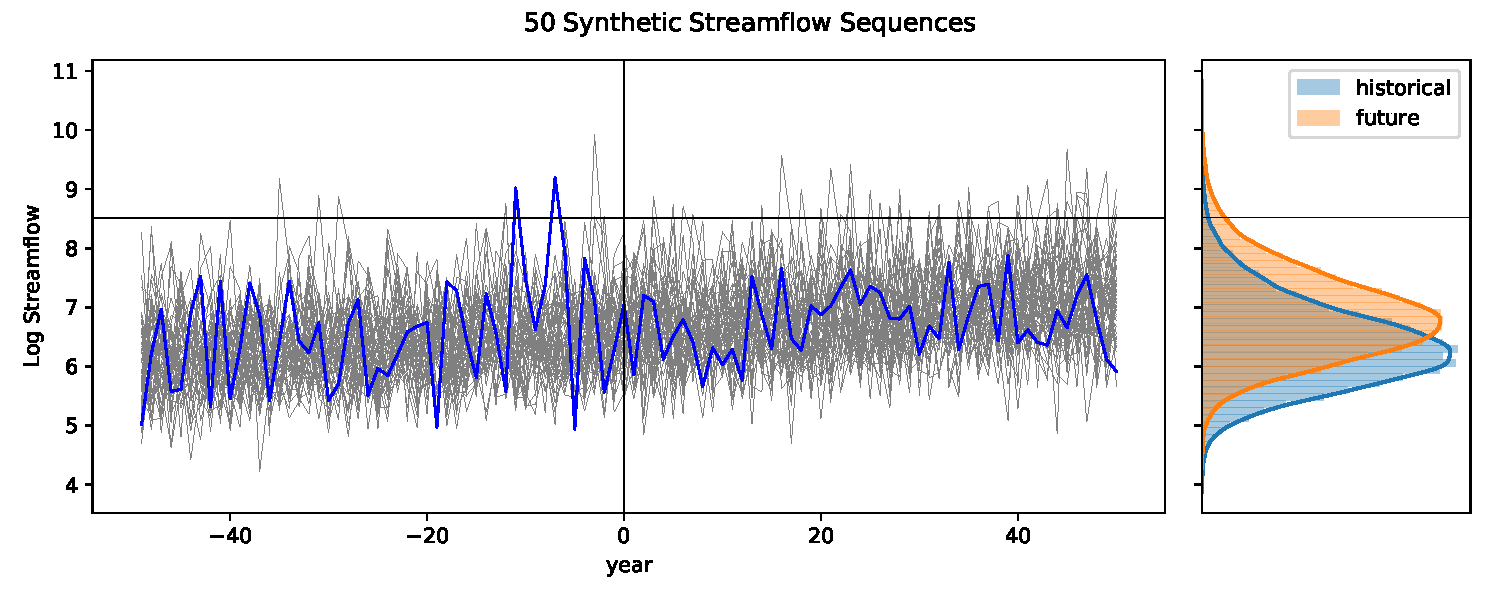
\includegraphics[width=\textwidth]{../../figs/trend_sequences.pdf}
  \caption{As \cref{fig:stationary-sequences} except \(\gamma=0.01\).}
\end{figure}

\section{Stationary, Static Risk}

Consider static risk and a stationary process, and partiuclarly implications of \(\qty{M, N}\).
Much of this is already laid out in \citet{Lall1987}.

\section{Stationary, Static Risk}

Consider static risk and a non-stationary process.
Estimate using drift or nonstationary models using full \(N\) of the most recent \(N\) (\ie{} what Vogel is proposing).
Illustrate via simulation for different signal to noise ratio of nonstationary terms and \(\qty{M, N}\).

\section{Dynamic Risk}

Consider dynamic risk, \ie{} updating and sequential decisions, a nonstationary generative process, and \(M\) and \(N\) considerations.

\section{Discussion}

Hopefully something to discuss?

\section{Summary}

Some interesting conclusions

\section{Notation}

\begin{description}
  \item[$Q$] Annual-maximum flood series
  \item[$Q_T$] Flood threshold
\end{description}


% -----------------------------------------------------------------------------
% END HERE
% -----------------------------------------------------------------------------
\clearpage
\printbibliography{}

\end{document}
